\documentclass[10pt,a4paper]{article}
\usepackage{tocloft}
\usepackage{commons/course}
\usepackage{booktabs}
\usepackage{graphicx}
\usepackage{tikz}
\usetikzlibrary{arrows.meta,positioning,calc,decorations.pathreplacing,fit}

\definecolor{keywordstyle}{rgb}{0.0, 0.4, 0.8}
\definecolor{stringstyle}{rgb}{0.9, 0.17, 0.31}
\definecolor{commentstyle}{rgb}{0.1, 0.6, 0.2}
\definecolor{numberstyle}{rgb}{0.4, 0.4, 0.4}
\definecolor{backgroundcolor}{rgb}{0.94, 0.97, 1.0}

\lstdefinelanguage{ShellLike}{
	morekeywords={PASS,FAIL,Passed,Failed,Running,Loading,summary,iverilog},
	sensitive=false,
	morecomment=[l]{\#},
	morestring=[b]",
}

\lstset{
	language=ShellLike,
	basicstyle=\ttfamily\scriptsize,
	keywordstyle=\color{keywordstyle}\bfseries,
	stringstyle=\color{stringstyle},
	commentstyle=\color{commentstyle},
	numbers=none,
	keepspaces=true,
	tabsize=2,
	showspaces=false,
	showstringspaces=false,
	showtabs=false,
	breaklines=true,
	breakatwhitespace=false,
	frame=single,
	backgroundcolor=\color{backgroundcolor},
}

\lstdefinestyle{verilog}{
	language=Verilog,
	basicstyle=\ttfamily\scriptsize,
	keywordstyle=\color{keywordstyle}\bfseries,
	commentstyle=\color{commentstyle},
	stringstyle=\color{stringstyle},
	numbers=left,
	numberstyle=\tiny\color{numberstyle},
	frame=single,
	backgroundcolor=\color{backgroundcolor},
	breaklines=true,
	tabsize=2,
}

\newlistof{listofproblems}{lop}{\normalsize فهرست مسائل}
\newcommand{\addproblem}[1]{\addcontentsline{lop}{listofproblems}{\protect\numberline{}#1}}

\begin{document}

\سربرگ{آزمایش پنجم}{طراحی ضرب‌کننده (روش \lr{Booth})}{}{استاد: دکتر انصاری}

\subsubsection*{خلاصه}

در این آزمایش یک واحد ضرب‌کننده‌ی علامت‌دار با روش {بوث} (\lr{Booth}) طراحی شده است. طبق خواسته‌ی صورت آزمایش، مسیرداده (\lr{datapath}) و واحد کنترل (\lr{control unit}) به‌صورت {جداگانه} طراحی و سپس در یک ماژول سطح‌بالا به یکدیگر متصل شده‌اند.

نکته‌ی کلیدی صورت آزمایش این است که واحد شیفت‌دهنده باید بتواند {بیش از یک بیت در هر پالس ساعت} شیفت بدهد تا نسبت به ضرب عادی (\lr{Shift \& Add}) تسریع داشته باشد. برای برآورده‌کردن این شرط، از {بوث پایه ۴} (\lr{radix-4} یا \lr{modified Booth}) استفاده شده است که در هر تکرار {دو بیت} از مضروب‌فیه را مصرف می‌کند و مجموعه‌ی $\{A, Q, Q_{-1}\}$ را {دو بیت به راست} شیفت می‌دهد. نتیجه این است که برای عملوند $N$ بیتی به جای $N$ تکرار، تنها $N/2$ تکرار لازم است.

صحت‌سنجی با \lr{Icarus Verilog} انجام شده و ضرب‌کننده روی {تمام} فضای ورودی علامت‌دار ۸ در ۸ بیت (هر $256 \times 256 = 65536$ جفت) با عملگر ضرب علامت‌دار خود \lr{Verilog} مقایسه شده است.

\subsubsection*{چرا پایه ۴؟}

در روش \lr{Shift \& Add} معمولی و همچنین بوث پایه ۲، در هر پالس ساعت تنها {یک} بیت از مضروب‌فیه بررسی و یک بیت شیفت انجام می‌شود؛ پس ضرب دو عدد $N$ بیتی $N$ کلاک طول می‌کشد.

در بوث پایه ۴، در هر تکرار یک پنجره‌ی {سه‌بیتی} از $\{Q_1, Q_0, Q_{-1}\}$ بررسی می‌شود و بر اساس آن یکی از پنج مضرب $\{0, +M, -M, +2M, -2M\}$ به انباشتگر اضافه می‌شود، سپس شیفت {دو بیتی} انجام می‌گیرد. جدول بازکدگذاری (\lr{recoding}) به این صورت است:

\begin{center}
\begin{tabular}{@{}ll ccc@{}}
\toprule
{تفسیر} & {عملیات} & $Q_{-1}$ & $Q_0$ & $Q_1$ \\
\midrule
دنباله‌ی صفر       & $A \mathrel{+}= 0$  & 0 & 0 & 0 \\
پایان دنباله‌ی یک  & $A \mathrel{+}= M$  & 1 & 0 & 0 \\
یک تکی             & $A \mathrel{+}= M$  & 0 & 1 & 0 \\
پایان دنباله‌ی یک  & $A \mathrel{+}= 2M$ & 1 & 1 & 0 \\
آغاز دنباله‌ی یک   & $A \mathrel{-}= 2M$ & 0 & 0 & 1 \\
صفر تکی            & $A \mathrel{-}= M$  & 1 & 0 & 1 \\
آغاز دنباله‌ی یک   & $A \mathrel{-}= M$  & 0 & 1 & 1 \\
دنباله‌ی یک        & $A \mathrel{+}= 0$  & 1 & 1 & 1 \\
\bottomrule
\end{tabular}
\end{center}

مقایسه‌ی تعداد کلاک‌ها که در تست‌بنچ هم {اندازه‌گیری} شده است:

\begin{center}
\begin{tabular}{@{}crrr@{}}
\toprule
$N$ & {پایه ۲ / \lr{Shift \& Add}} & {پایه ۴ (این طراحی)} & {تسریع} \\
\midrule
۴  & ۵ کلاک  & ۳ کلاک & $1.7\times$ \\
۸  & ۹ کلاک  & ۵ کلاک & $1.8\times$ \\
۱۶ & ۱۷ کلاک & ۹ کلاک & $1.9\times$ \\
\bottomrule
\end{tabular}
\end{center}

اعداد ستون سوم مستقیما از خود مدار خوانده شده‌اند، نه اینکه فرض شده باشند؛ تست‌بنچ لبه‌های کلاک را تا فعال‌شدن \lr{done} می‌شمارد.

\subsubsection*{معماری کلی}

طراحی از سه ماژول تشکیل شده است:

\begin{center}
\begin{latin}
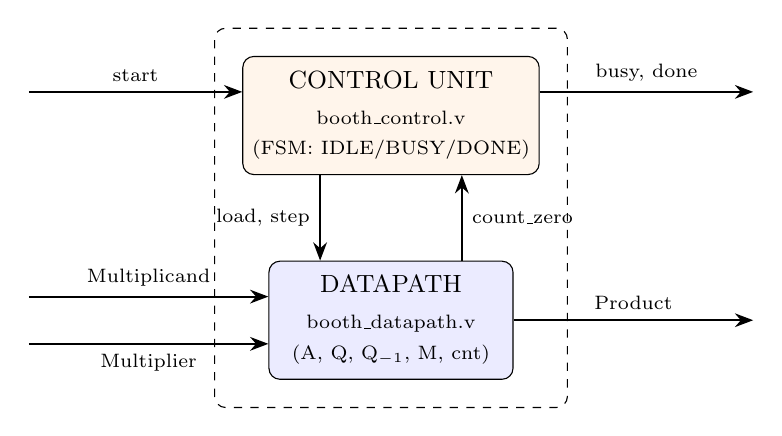
\begin{tikzpicture}[
  blk/.style={draw, rounded corners, minimum width=3.1cm, minimum height=1.5cm, align=center, font=\small},
  >=Stealth
]
  \node[blk, fill=orange!8] (cu) at (0,2.6) {CONTROL UNIT\\[2pt]\scriptsize booth\_control.v\\\scriptsize (FSM: IDLE/BUSY/DONE)};
  \node[blk, fill=blue!8]   (dp) at (0,0)   {DATAPATH\\[2pt]\scriptsize booth\_datapath.v\\\scriptsize (A, Q, Q$_{-1}$, M, cnt)};

  \draw[->, thick] ($(cu.south)+(-0.9,0)$) -- ($(dp.north)+(-0.9,0)$)
        node[midway, left, font=\scriptsize] {load, step};
  \draw[->, thick] ($(dp.north)+(0.9,0)$) -- ($(cu.south)+(0.9,0)$)
        node[midway, right, font=\scriptsize] {count\_zero};

  \draw[->, thick] (-4.6,2.9) -- (cu.west |- 0,2.9) node[midway, above, font=\scriptsize] {start};
  \draw[->, thick] (cu.east |- 0,2.9) -- (4.6,2.9)  node[midway, above, font=\scriptsize] {busy, done};

  \draw[->, thick] (-4.6,0.3) -- (dp.west |- 0,0.3) node[midway, above, font=\scriptsize] {Multiplicand};
  \draw[->, thick] (-4.6,-0.3) -- (dp.west |- 0,-0.3) node[midway, below, font=\scriptsize] {Multiplier};
  \draw[->, thick] (dp.east |- 0,0) -- (4.6,0) node[midway, above, font=\scriptsize] {Product};

  \node[draw, dashed, rounded corners, inner sep=10pt, fit=(cu)(dp)] {};
\end{tikzpicture}
\end{latin}
\end{center}

\begin{center}
\begin{tabular}{@{}l p{9.2cm}@{}}
\toprule
{ماژول} & {مسئولیت} \\
\midrule
\lr{booth\_datapath.v}   & همه‌ی رجیسترها و محاسبات: انباشتگر $A$، مضروب‌فیه $Q$، بیت $Q_{-1}$، مضروب $M$، شمارنده، بازکدگذاری بوث و شیفت دوبیتی. هیچ تصمیم ترتیبی نمی‌گیرد. \\
\lr{booth\_control.v}    & ماشین حالت \lr{Moore} با سه حالت. فقط تعیین می‌کند {چه زمانی} عملوندها بارگذاری و {چه زمانی} یک تکرار اجرا شود. هیچ داده‌ای نگه نمی‌دارد. \\
\lr{booth\_multiplier.v} & اتصال این دو به یکدیگر؛ خودش منطقی ندارد. \\
\bottomrule
\end{tabular}
\end{center}

\subsubsection*{مشخصات واسط}

\begin{center}
\begin{tabular}{@{}lll p{6.6cm}@{}}
\toprule
{سیگنال} & {جهت} & {پهنا} & {توضیح} \\
\midrule
\lr{Clk}          & ورودی & ۱     & کلاک؛ لبه‌ی بالارونده \\
\lr{RstN}         & ورودی & ۱     & ریست ناهم‌گام فعال‌پایین \\
\lr{start}        & ورودی & ۱     & درخواست شروع یک ضرب جدید \\
\lr{Multiplicand} & ورودی & $N$   & مضروب (علامت‌دار، مکمل ۲) \\
\lr{Multiplier}   & ورودی & $N$   & مضروب‌فیه (علامت‌دار، مکمل ۲) \\
\lr{Product}      & خروجی & $2N$  & حاصل‌ضرب علامت‌دار \\
\lr{busy}         & خروجی & ۱     & ۱ یعنی ضرب در جریان است \\
\lr{done}         & خروجی & ۱     & ۱ یعنی نتیجه آماده است \\
\bottomrule
\end{tabular}
\end{center}

سیگنال \lr{done} از نوع {سطح} است و تا رسیدن \lr{start} بعدی بالا می‌ماند، بنابراین یک مصرف‌کننده‌ی کند هم نتیجه را از دست نمی‌دهد.

\subsubsection*{مسیرداده}



نکته‌ای که در پیاده‌سازی اهمیت زیادی دارد {پهنای انباشتگر} است. در بسیاری از توضیحات درسی، $A$ را $N+1$ بیت می‌گیرند؛ اما در پایه ۴ این کافی نیست. اگر مضروب برابر منفی‌ترین مقدار ممکن یعنی $M = -2^{N-1}$ باشد، آنگاه:

\[
2M = -2^{N} \qquad\text{و}\qquad -2M = +2^{N}
\]

مقدار $+2^{N}$ در $N+1$ بیت علامت‌دار {جا نمی‌شود} (بازه‌ی آن $[-2^{N},\, 2^{N}-1]$ است). بنابراین در این طراحی $A$ و مقدار افزودنی هر دو $N+2$ بیت گرفته شده‌اند تا هر پنج مضرب دقیقا نمایش‌پذیر باشند و منفی‌ترین عملوند نیازی به حالت خاص نداشته باشد.


\begin{latin}
\lstinputlisting[style=verilog]{../rtl/booth_datapath.v}
\end{latin}

\subsubsection*{واحد کنترل}

واحد کنترل یک ماشین حالت \lr{Moore} با سه حالت است:

\begin{center}
\begin{latin}
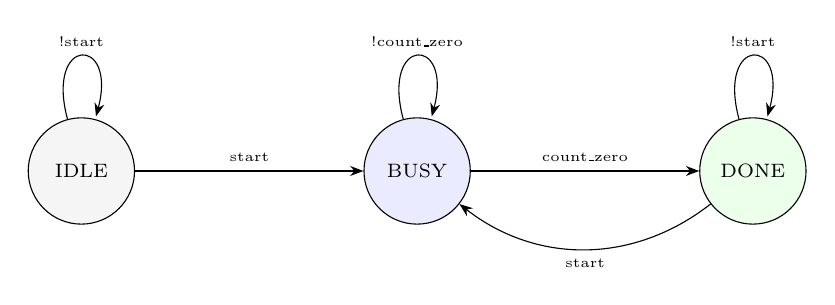
\begin{tikzpicture}[
  st/.style={draw, circle, minimum size=1.35cm, align=center, font=\scriptsize},
  >=Stealth, node distance=2.9cm
]
  \node[st, fill=black!4] (idle) {IDLE};
  \node[st, fill=blue!8, right=of idle] (busy) {BUSY};
  \node[st, fill=green!8, right=of busy] (done) {DONE};

  \draw[->] (idle) -- (busy) node[midway, above, font=\tiny] {start};
  \draw[->] (busy) -- (done) node[midway, above, font=\tiny] {count\_zero};
  \draw[->] (busy) edge[loop above] node[font=\tiny] {!count\_zero} (busy);
  \draw[->] (idle) edge[loop above] node[font=\tiny] {!start} (idle);
  \draw[->] (done) edge[loop above] node[font=\tiny] {!start} (done);
  \draw[->] (done) to[bend left=38] node[midway, below, font=\tiny] {start} (busy);
\end{tikzpicture}
\end{latin}
\end{center}

\begin{center}
\begin{tabular}{@{}l l l p{5.4cm}@{}}
\toprule
{حالت} & \lr{load} & \lr{step} & {توضیح} \\
\midrule
\lr{IDLE} & \lr{start} & 0 & منتظر درخواست؛ با \lr{start} عملوندها بارگذاری می‌شوند \\
\lr{BUSY} & 0 & 1 & در هر کلاک یک تکرار پایه ۴ اجرا می‌شود \\
\lr{DONE} & \lr{start} & 0 & نتیجه معتبر است و تا \lr{start} بعدی می‌ماند \\
\bottomrule
\end{tabular}
\end{center}

توجه کنید که واحد کنترل خودش شمارنده ندارد؛ شمارنده در مسیرداده است و کنترل فقط پرچم وضعیت \lr{count\_zero} را می‌بیند. این تفکیک باعث می‌شود تغییر عمق تکرار (مثلا با تغییر $N$) هیچ اثری روی واحد کنترل نداشته باشد.

\begin{latin}
\lstinputlisting[style=verilog]{../rtl/booth_control.v}
\end{latin}

\subsubsection*{اتصال دو واحد}

ماژول سطح‌بالا فقط این دو را به هم وصل می‌کند و منطق مستقلی ندارد:

\begin{latin}
\lstinputlisting[style=verilog]{../rtl/booth_multiplier.v}
\end{latin}

\subsubsection*{شکل موج}

شکل‌موج دو ضرب پشت‌سرهم را نشان می‌دهد: ابتدا $25 \times (-7) = -175$ و سپس $(-12) \times (-11) = +132$؛ یعنی هر دو حالت افزودن و کاستن در بازکدگذاری بوث دیده می‌شود.

\begin{center}
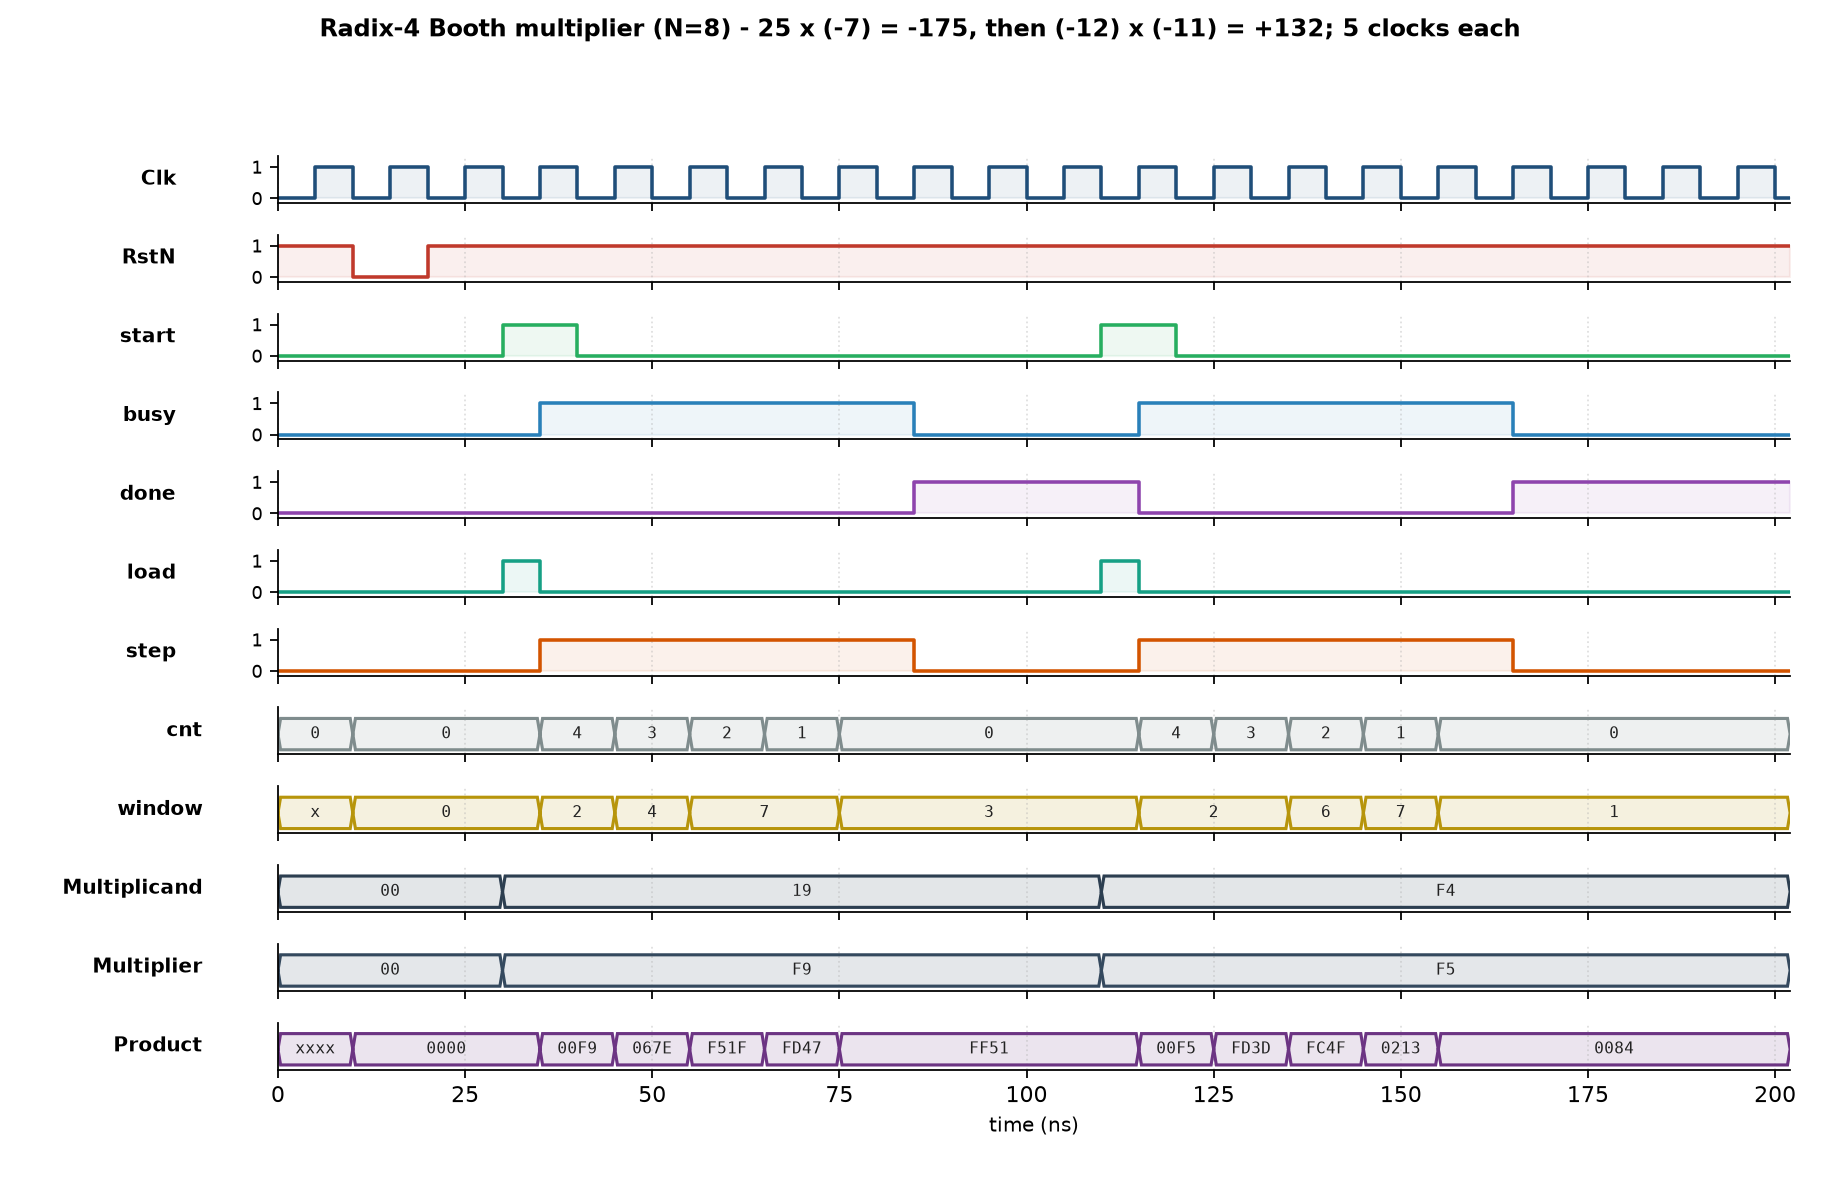
\includegraphics[width=\textwidth]{figs/wave_booth.png}\\[0.4em]
\end{center}

نکات قابل مشاهده در شکل: شمارنده‌ی \lr{cnt} دنباله‌ی $4 \to 3 \to 2 \to 1 \to 0$ را طی می‌کند، یعنی دقیقا {چهار} تکرار برای عملوند ۸ بیتی و نه هشت تکرار. سیگنال \lr{window} همان پنجره‌ی سه‌بیتی است که در هر تکرار عوض می‌شود. مقدار \lr{Product} در پایان ضرب اول برابر \lr{FF51} است که در مکمل ۲ همان $-175$ می‌شود، و در پایان ضرب دوم \lr{0084} یعنی $+132$. همچنین دیده می‌شود که \lr{load} تنها یک پالس تک‌کلاکی است در حالی که \lr{step} در سراسر حالت \lr{BUSY} فعال می‌ماند.

\subsubsection*{تست‌بنچ اصلی}

تست‌بنچ اصلی حاصل‌ضرب را با عملگر ضرب {علامت‌دار} خود \lr{Verilog} مقایسه می‌کند و کل فضای ورودی ۸ در ۸ بیت را به‌صورت \lr{exhaustive} می‌پیماید. علاوه بر آن، حالت‌های مرزی کلاسیک به‌صورت جداگانه هم آزموده شده‌اند: صفرها، $\pm 1$، بزرگ‌ترین مثبت‌ها، منفی‌ترین مقدار $-128$ (از جمله $-128 \times -128$)، الگوهای متناوب \lr{0x55}/\lr{0xAA}، شروع‌های پشت‌سرهم بدون ریست، و ریست در {میانه‌ی} یک ضرب.

\begin{latin}
\lstinputlisting[style=verilog]{../tb/tb_booth_multiplier.v}
\end{latin}

\subsubsection*{تست‌بنچ پارامتری و اندازه‌گیری تسریع}

تست‌بنچ دوم دو کار انجام می‌دهد که تست اول انجام نمی‌دهد. اول اینکه همان ماژول را با سه پهنای متفاوت ($N = 4, 8, 16$) می‌سازد تا مطمئن شویم هیچ‌جای طراحی به عدد ۸ گره نخورده است. دوم اینکه تعداد کلاک هر ضرب را از خود مدار {اندازه می‌گیرد} و بررسی می‌کند که واقعا برابر $N/2 + 1$ باشد؛ یعنی ادعای شیفت بیش از یک بیت در هر کلاک به‌صورت عددی اثبات می‌شود نه اینکه صرفا ادعا شود.

\begin{latin}
\lstinputlisting[style=verilog]{../tb/tb_booth_param.v}
\end{latin}

\subsubsection*{نتایج تست}

\begin{latin}
\lstinputlisting[basicstyle=\ttfamily\scriptsize]{figs/test_run_output.txt}
\end{latin}

\subsubsection*{جمع‌بندی}

در این آزمایش دیدیم که تفکیک {مسیرداده} از {واحد کنترل} چه فایده‌ای دارد. مسیرداده فقط می‌داند چگونه یک تکرار بوث را انجام دهد و واحد کنترل فقط می‌داند چند بار و چه زمانی این کار باید تکرار شود. نتیجه این است که هیچ‌کدام به جزئیات دیگری وابسته نیستند؛ مثلا تغییر $N$ از ۸ به ۱۶ فقط تعداد تکرارها را عوض می‌کند و یک خط از واحد کنترل هم تغییر نمی‌کند.

درباره‌ی شرط تسریع، استفاده از بوث پایه ۴ باعث شد تعداد کلاک‌ها از $N+1$ به $N/2+1$ کاهش پیدا کند، یعنی حدود دو برابر سریع‌تر. البته این تسریع رایگان نیست: در ازای آن باید یک جمع‌کننده‌ی پهن‌تر و منطق انتخاب پنج‌حالته برای مضرب‌ها پرداخت شود، که مصالحه‌ی همیشگی {سرعت در برابر سطح} است.

\pagebreak
\subsubsection*{خروجی سنتز (\lr{Quartus Prime})}

طرح روی \lr{Intel Quartus Prime Lite Edition 21.1.0} با موجودیت سطح‌بالای \lr{booth\_multiplier} سنتز و Place \& Route شد. دستگاه هدف: \lr{Cyclone V} (\lr{5CGXFC7C7F23C8}).

\begin{center}
\begin{tabular}{@{}lr@{}}
\toprule
{مورد} & {نتیجه} \\
\midrule
وضعیت کامپایل & موفق ($0$ خطا، $13$ هشدار) \\
\lr{Logic utilization (ALMs)} & $28 / 56480$ ($<1\%$) \\
\lr{Total registers} & $30$ \\
\lr{Total pins} & $37 / 268$ ($14\%$) \\
\lr{Block memory bits} & $0$ \\
\lr{DSP Blocks} & $0$ \\
\bottomrule
\end{tabular}
\end{center}

\begin{center}

\includegraphics[width=\textwidth]{figs/quartus_synthesis.jpg}
\end{center}

\end{document}
